\subsection{Range of Classification Algorithms}
\label{subsec:algorithm-exploration}

Having selected supervised classification, the next question is which
algorithm offers an appropriate balance of discrimination, case detection,
and interpretability for a small tabular dataset.
Table~\ref{tab:classification-algorithms} distinguishes the algorithms
implemented in the Python experiments from alternatives considered on
methodological grounds. Unimplemented alternatives are not claimed to have
been empirically outperformed.

\begin{table}[H]
\centering
\small
\caption{Algorithm-level exploration within supervised classification.}
\label{tab:classification-algorithms}
\begin{tabularx}{\textwidth}{@{}p{2.7cm}XX@{}}
\toprule
Algorithm & Strength and limitation & Role in this iteration \\
\midrule
Logistic regression &
Regularised, interpretable probability model; its additive form can miss
interactions unless represented in the predictors. &
Implemented as the principal baseline. Despite its name, it models a binary
class probability here. \\
Decision trees: CART &
Readable nonlinear rules, but individual trees can be unstable and overfit
small samples. &
CART is used for feature selection; \\
Random forest &
Combines trees to model interactions; less transparent than a single tree,
with potentially misleading impurity importance for correlated predictors. &
Implemented as the bagged-tree alternative. \\
XGBoost and LightGBM &
Boosted trees can capture nonlinear structure; complexity requires control
through tree size, learning rate, and regularisation. &
Both implemented with bounded settings and tuning grids. \\
Support vector machine &
Linear or kernel boundaries offer alternatives to additive probabilities;
scaling, kernel choice, and probability estimation add decisions. &
Considered but not implemented in this bounded Python comparison. Earlier
test-set LSVM results are not a selection justification. \\
$k$-nearest neighbours and naive Bayes &
Neighbour methods are sensitive to scaling and redundant dimensions;
naive Bayes is simple but assumes conditional independence. &
Not implemented; correlated measurements make their assumptions or distance
representation worth further investigation rather than automatic adoption. \\
Neural network &
Can represent complex interactions, but adds architecture and optimisation
choices and is harder to interpret. &
Deferred given the sample size and scope; no claim that it cannot perform
competitively. \\
Stacking &
Combines complementary model probabilities; requires out-of-fold training
and increases fitting and explanation costs. &
Implemented using the four individual predictive models and a logistic
meta-classifier. \\
\bottomrule
\end{tabularx}
\end{table}

This candidate set tests whether nonlinear models or their combination improve
on the simpler baseline. A training-prior dummy classifier provides a
feature-free benchmark. Unsupervised algorithms are not additional candidates
for the final classifier; their exploratory role is established in
Section~\ref{subsec:dm-family-comparison}.

\subsection{Model Construction Protocol}
\label{subsec:python-candidate-construction}

The Open Source Software Stack uses Python/Jupyter, pandas and NumPy,
scikit-learn, XGBoost, LightGBM, and plotting libraries. Shared
\path{utils.py} and \path{modeling.py} functions support the transformation,
holdout, leave-one-out, tuning, and error-analysis notebooks.

Five label-stratified splits (seeds 42, 7, 21, 84, and 123) each produce
223 training, 48 validation, and 48 test rows. Within training, continuous
measurements are median-imputed and categorical fields most-frequent-imputed.
RFE with CART or direct CART importance selects 20 source predictors, followed
by Yeo--Johnson and standardisation for continuous fields and one-hot encoding
for categories. CART selection uses maximum depth 5 and minimum leaf size 4;
RFE removes one feature per step. The complete preparation is refitted inside
inner CV, including stacking's base pipelines. The globally transformed
reference CSV is not an evaluation input.

\subsection{Parameter Settings, Rationale and Tested Alternatives}
\label{subsec:parameter-settings}

\begin{table}[H]
\centering
\small
\caption{Implemented fixed settings and training-only search spaces.}
\label{tab:python-parameters}
\begin{tabularx}{\textwidth}{@{}p{2.5cm}XX@{}}
\toprule
Model & Fixed settings & Tuning grid \\
\midrule
Logistic regression &
$C=1$; maximum 3,000 iterations. &
$C\in\{0.1,1,10\}$. \\
Random forest &
60 trees; maximum depth 5; minimum leaf size 4. &
Depth $\{3,5,8\}$; leaf size $\{2,4\}$. \\
XGBoost &
60 trees; learning rate 0.05; depth 2; $\lambda=1$; row/column sampling 0.8;
histogram tree method. &
Depth $\{2,3\}$; learning rate $\{0.03,0.05\}$. \\
LightGBM &
60 trees; learning rate 0.05; 7 leaves; minimum child samples 20;
column sampling 0.8. &
Leaves $\{7,15\}$; learning rate $\{0.03,0.05\}$. \\
Stacking &
Three stratified inner folds; probability inputs; standardised logistic
meta-model, $C=1$, maximum 3,000 iterations; no raw-feature passthrough. &
Fixed benchmark, not tuned. \\
\bottomrule
\end{tabularx}
\end{table}

The tuning notebook fixes RFE--CART and uses three-fold stratified
\texttt{GridSearchCV} within training to select each family's parameters by
mean ROC--AUC. Validation then selects the model family. These limited grids
control experiment scope; they do not establish globally optimal settings.


\paragraph{Rationale and limits of the choices.}
Logistic regression's $C=1$ provides a regularised reference; the tested
$C=0.1$ and $C=10$ alternatives increase and decrease regularisation.
The 3,000-iteration limit provides optimisation headroom, not additional
model capacity. Random forest depth 5 and leaf size 4 limit small-sample
fragmentation; depths 3 and 8 and leaf size 2 test that restriction.
For XGBoost, depth 2 restricts interaction complexity, learning rate 0.05
shrinks each update, and row/column sampling 0.8 reduces reliance on any one
subset. Its depth and learning-rate alternatives test capacity and shrinkage.
LightGBM's 7 leaves and minimum child size 20 limit small terminal groups;
15 leaves and learning rate 0.03 test alternatives. The shared 60-tree budget
bounds computation; its optimality was not tested. XGBoost's $\lambda=1$
and histogram method, and the sampling fractions, remain fixed controls
rather than empirically optimised choices.

Stacking uses three stratified folds to construct out-of-fold probability
inputs within the training data. A standardised logistic meta-model with
$C=1$ and no raw-feature passthrough limits the second-stage input space.
The fold count and meta-model settings were not tuned. CART selection's
depth 5 and leaf size 4 similarly constrain small-sample splits; RFE removes
one field at a time to reach 20. Section~\ref{subsec:iterations} tests the
alternative of 10 fields. The 0.5 threshold is a fixed reference, not a
sensitivity-optimised operating point. These distinctions separate tested
choices from settings that still require investigation.

\begin{table}[H]
\centering\small
\caption{Executed training-CV alternatives: seed 42, RFE--CART. Winning configurations are selected within each family; scores are not test results.}
\begin{tabular}{lp{0.8cm}p{6.5cm}r}
\toprule
Model & Trials & Best tested settings & CV AUC \\
\midrule
Logistic regression & 3 & C=0.1 & 0.8716 \\
Random forest & 6 & max depth=5, min samples leaf=2 & 0.8475 \\
XGBoost & 4 & learning rate=0.05, max depth=3 & 0.8446 \\
LightGBM & 4 & learning rate=0.03, num leaves=7 & 0.8485 \\
\bottomrule
\end{tabular}
\end{table}

Across seeds 42, 7, 21, 84 and 123, the selected logistic $C$ values are 0.1, 0.1, 0.1, 1 and 10. The figure below exposes the actual seed-42 alternatives, rather than only listing a proposed search grid. Source: \path{results/tuning/seed_42_*_cv.csv}.


\begin{figure}[H]
\centering
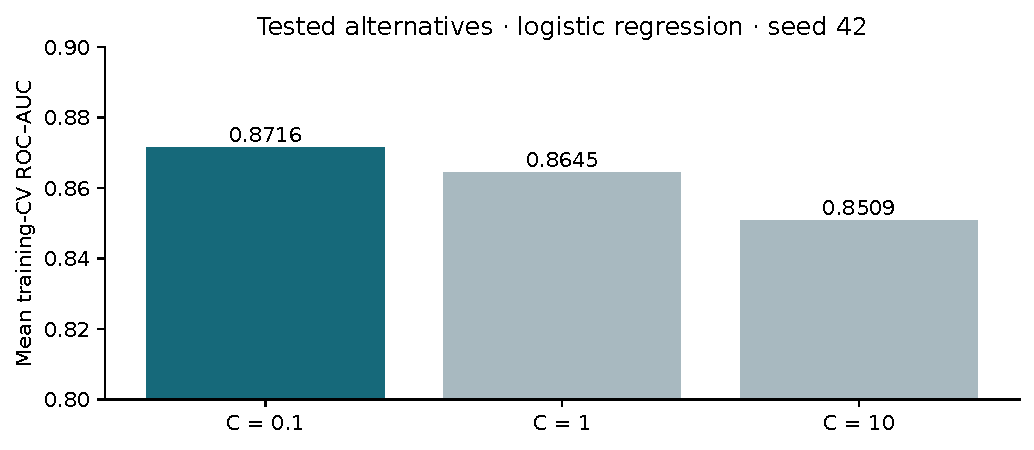
\includegraphics[width=0.88\textwidth]{figures/modeling/parameter_search.pdf}
\caption{Executed logistic-regression parameter alternatives for seed 42.
Scores are means over three training CV folds from the saved search output;
validation and test scores are not used in this parameter comparison.}
\label{fig:parameter-search}
\end{figure}
